\section{ Descripción del problema }

El perfil parabólico de velocidad que resulta de un fluido que circula dentro de una tubería de sección circular se puede calcular analíticamente (Ley de Poiseuille). Este perfil se obtiene por la acción de los esfuerzos cortantes debido a la viscosidad del fluido. La ecuación que describe este perfil viene dada por:

\begin{equation}
u = \dfrac{\Delta P}{4 \mu L } \left( R^2 - r^2 \right)
\end{equation} 

donde $\Delta P$ es el gradiente de presión entre ambos extremos de la tubería, $\mu$ es la viscosidad dinámica, $L$ y $R$ corresponde a la longitud y al radio de la tubería, $r \in [0,R]$ es una posición dentro de la tubería.

\subsection{Dominio físico y numérico}

Se estudia el comportamiento de un fluido en tubería de radio $L_y$ y longitud $L_x$. Su modelo discretizado se representa mediante una malla regular desplazada (ver Figura \ref{malla}). Los puntos negros corresponden a las coordenadas de la presión (o de escalar pasivo $\phi$) y los puntos azules y rojos a las componentes horizontales y verticales de la velocidad, respectivamente. \\ 

Para facilitar el procedimiento de resolución, se incluyen nodos ficticios en la discretización, representados por los volúmenes de color ( $ i=1,ny+2 $ para $ j=1 $ y $j=nx+2$ ;  $ j=1,nx+2 $ para $ i=1 $ e $i=ny+2$ ) que contienen las condiciones de contorno del problema. Notar de la Figura que las variables $u(i,j=1)$ y $v(i=ny+2,j)$ no aportan información al problema, pero se conservan para respetar la nomenclatura de los puntos de la malla.

\begin{center}
\begin{figure}
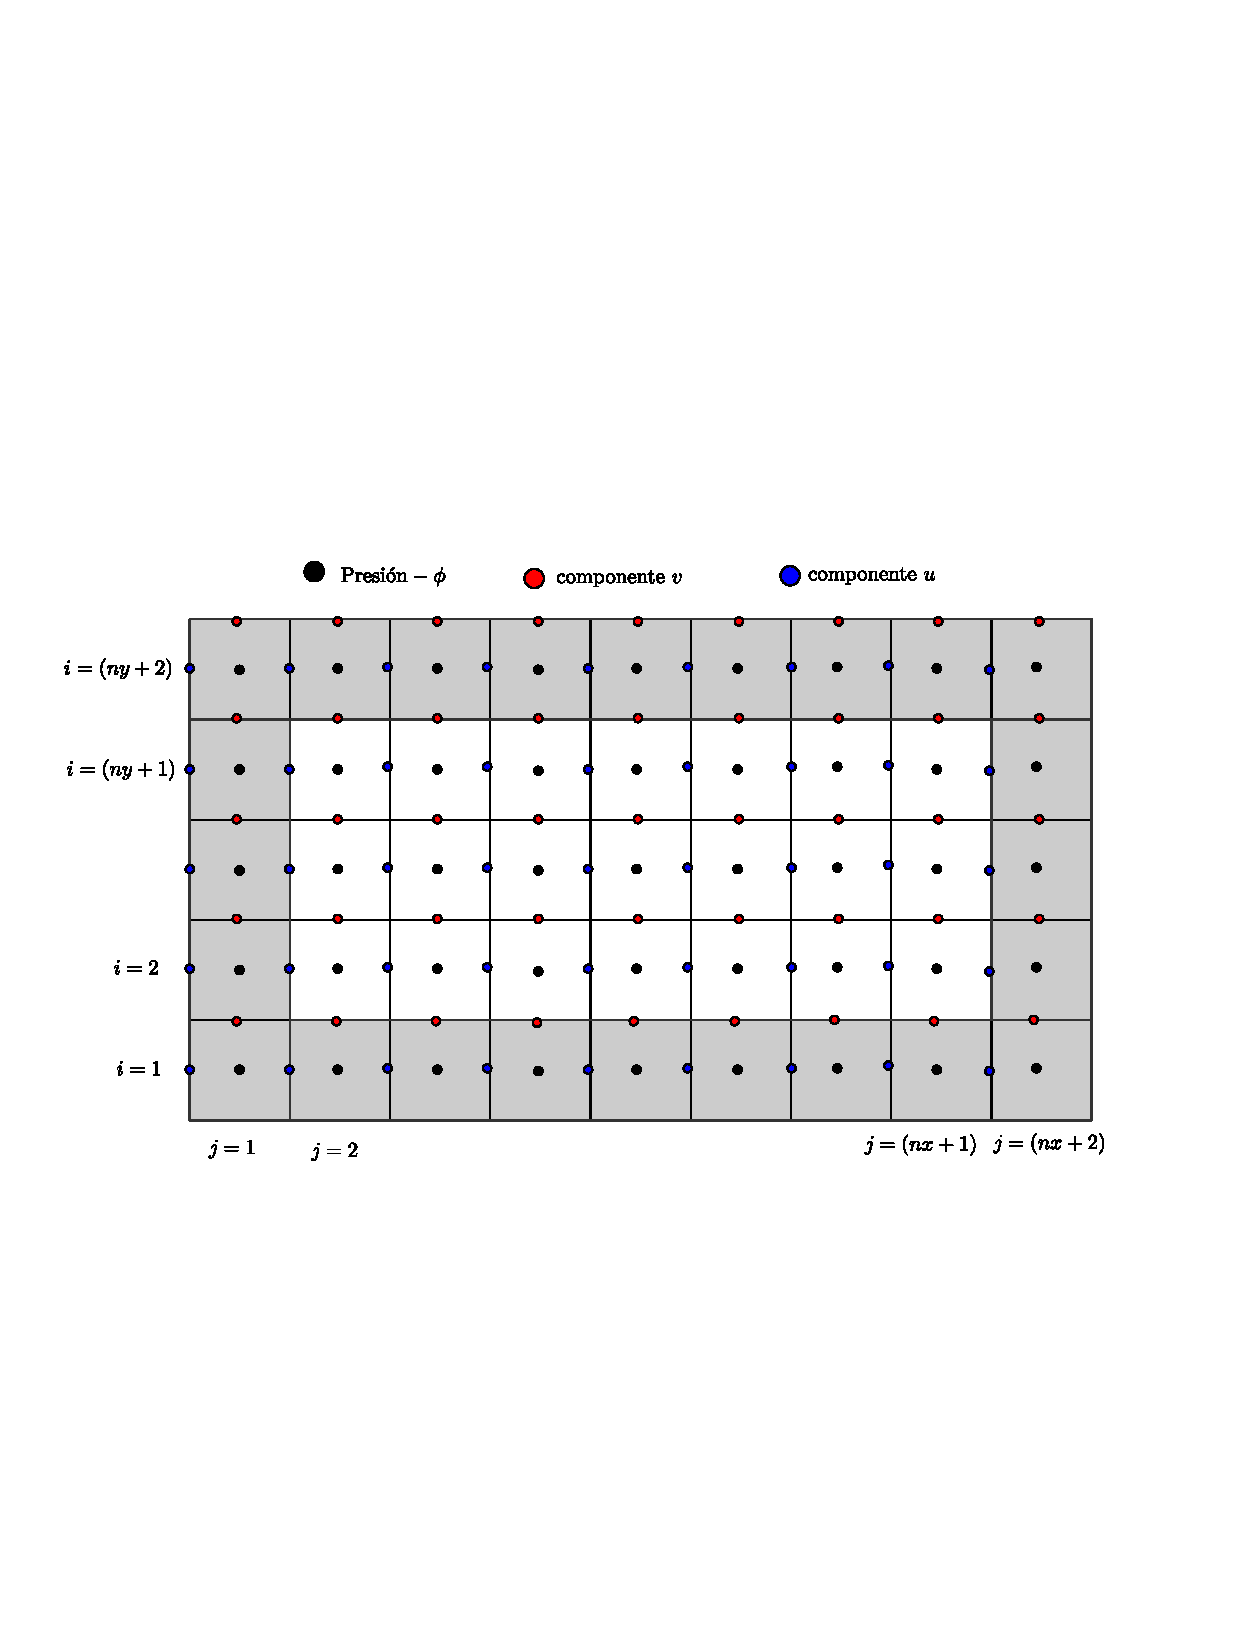
\includegraphics[width=1\textwidth]{malla.png}
\caption{Malla regular de discretización del dominio} \label{malla}
\end{figure}
\end{center}

\subsection{Algoritmo de resolución}

En la Figura \ref{algoritmo} se muestra un diagrama de flujo del código implementado. El preámbulo (dimensiones, número de nodos, parámetros físicos, etc.) está incluido de un módulo. 

\begin{enumerate}
\item Inicio programa \texttt{CFD\_POISEUILLE} (Preámbulo contenido en el módulo)
\item Se imponen las condiciones iniciales
\item Se imponene las condiciones de contorno
\item \label{iter} Inicio de la iteración de $k$ desde 1 a $nt$ ($nt$: número de pasos de tiempo)
\item \label{cor_vel} Se calcula la predicción de la velocidad
\item Se corrige la presión mediante la resolución de la ecuación de Poisson de $\phi$
\item Se verifica la convergencia de las variables. Si el término de fuente de masa o el número de iteraciones satisfacen cierto criterio, se regresa al paso \ref{cor_vel}. Caso contrario, continua con el siguiente paso
\item Se corrige el campo de velocidad
\item Se verifica si se logra un flujo estacionario. Si está en estado transiente, se imponen las condiciones de contorno y se vuelve al paso \ref{iter}. Caso contrario, se exportan los datos y se grafican.
\item Fin del programa \texttt{CFD\_POISEUILLE}
\end{enumerate}

\begin{center}
\begin{figure}
\includegraphics[width=1\textwidth]{diagrama_flujo_1.pdf}
\caption{Algoritmo de resolución para el problema de Poiseuille} \label{algoritmo}
\end{figure}
\end{center}

\paragraph{Condiciones de contorno} Establece condición de no deslizamiento en la cara inferior (i=2,j) y simetría en la cara superior (i=ny+1,j). Se imponen condición de presión en la entrada y salida de la tubería, de tal manera de poder calcular directamente $\Delta P$ y poder comparar el perfil de velocidad con la solución analítica de Poiseuille.